\documentclass[12pt, a4paper,oneside, openany]{book}
%fuente12pt,tamaño carta,una cara,quitar hojas en blanco,tipo libro
\usepackage[utf8]{inputenc} %fuente Unicode
%\usepackage[margin=-0cm]{geometry} %margen
\usepackage{graphicx} %uso de imagenes
\usepackage{multicol} %uso de multicolumnas
\usepackage{multirow} %multi celdas
\usepackage{lastpage} %n.total de paginas
\usepackage{colortbl} %columnas de color
\usepackage{tikz, tikz-3dplot} %figuras
\usepackage{tkz-euclide}
\usepackage{adjustbox} %manejo de margenes
\usepackage[spanish]{babel} %lenguaje español
\usepackage[document]{ragged2e} %alineacion
\usepackage[T1]{fontenc} %codificacion fuente
\usepackage{palatino} %fuente
\usepackage{enumerate} %viñeta numeros
\usepackage[colorlinks,linkcolor=myblue,citecolor=mygreen]{hyperref} %link personalizado
%-------------------------------------------------------------------
\definecolor{myblue}{HTML}{2D74B5} %color de titulos y subtitulos
%-------------------------------------------------------------------
\graphicspath{ {img/} } %localizacion de carpeta con imagenes
\renewcommand{\baselinestretch}{1.2} %espacio entre parrafos

%\AtBeginDocument{\AtBeginShipoutNext{\AtBeginShipoutDiscard}}
%elimina paginas adicionales que se agregan con el uso de hyperref

\usepackage{multirow} %multi celdas en tablas
\usepackage{longtable} %tablas multipagina
\usepackage{caption} %ajuste de tablas, figuras
\usepackage{color} %colores de texto
\usepackage{wrapfig} %rodear imagenes
\usepackage{booktabs, multirow} %bordes y rangos
\usepackage{titlesec} %titulos personalizados
\usepackage{eso-pic,picture} %imagenes con texto
\usepackage{nomencl} %simbolos de nomenclatura
\usepackage{lipsum} %crea texto default
\makenomenclature %tamaño nomenclatura
%\usepackage{showframe} %muestra el margen de las pg
%-------------------------------------------------------------------
%codigo del borde
\AddToShipoutPicture{%
\setlength\fboxsep{1pt}%
\put(24pt,24pt){\framebox(19.3066cm,28.0066cm)[lb]{}}%
}

%margenes
\usepackage{geometry}
\newgeometry{
        top=0.001in,
        bottom=3.2in,
        outer=0.55in,  %izquierda
        inner=0.55in, %derecha
        }
%-------------------------------------------------------------------
\usepackage{fancyhdr}%uso de encabezado y pie personalizado
\pagestyle{fancy}

\setlength{\headheight}{160pt}%ubicacion de caja de encabezado

\titlespacing{\chapter}{0pt}{-42pt}{0.5cm}%config capitulos, espacio de chapter
\titleformat{\chapter}[display]
{\sffamily\color{myblue}} {
  {\normalfont\color{myblue}\Large}
        \hspace{0pt}
            {\setlength\fboxsep{0pt}
                \colorbox{myblue}{
                }
            }
    }
  {0 pt}
  {\titlerule[0pt]\LARGE\sffamily}

%-------------------------------------------------------------------
\fancyhf{}%Declaración de encabezado
\pagestyle{fancy}
\fancypagestyle{plain}{}
%encabezado general
\begin{document}%inicio de documento
\lhead{

\begin{minipage}{0.1\textwidth}
\scalebox{1}[1.2]{
\begin{tabular}{|m{2cm}|m{10.8cm}|m{1.0cm}|m{1.0cm}|m{1.0cm}| }

\hline

\multirow{3}{2cm}{\centering
\includegraphics[width=1.0\textwidth]{tjacdmx_logo.png}}
& \footnotesize\centering\bf\sffamily{TRIBUNAL DE JUSTICIA ADMINISTRATIVA DE TABASCO}
& \footnotesize\bf\sffamily{Día}
& \footnotesize\bf\sffamily{Mes}
&\footnotesize\bf\sffamily{Año}
\\ \cline{2-5}

& \centering\bf\footnotesize\sffamily{DIRECCIÓN GENERAL DE ADMINISTRACIÓN}
& \footnotesize\centering\bf\sffamily{28}
& \footnotesize\centering\bf\sffamily{02}
& \footnotesize\bf\sffamily{2023}
\\ \cline{2-5}

& \centering\bf\footnotesize\sffamily{DIRECCIÓN DE INFORMÁTICA}
& \multicolumn{3}{ |c| }{\bf\footnotesize\sffamily{Versión: 001 }}
\\ \cline{2-5}

&
\centering\bf\footnotesize\sffamily{MANUAL DE USUARIO}
& \multicolumn{3}{ |c| } {\bf\footnotesize\sffamily{Página \thepage~de\ \pageref{LastPage}}}
\\ \hline

\end{tabular}}
\end{minipage}

}
%-------------------------------------------------------------------

\centerline{
\includegraphics[width=0.8\textwidth]{tjacdmx_logo.png}}%imagen de logo en portada
%titulo de portada

\vspace{1cm}%espacio
%-------------------------------------------------------------------
\begin{flushright}%alineación a la derecha

\newcommand{\ProjectTitle}

\vspace{0cm}
%titulo en portada
{\color{myblue}{\sffamily\large\bf\sffamily
ACTUARIA\\
CONSULTA DE EXPEDIENTES\\
\vspace{0.6cm}
MANUAL DE USUARIO\\
\vspace{0.2cm}
DIRECCIÓN DE INFORMÁTICA}
}

\end{flushright}
%-------------------------------------------------------------------
%pie de todas las paginas
\cfoot[]{
{
\scalebox{1}[0.9]{%tamaño de celdas
\centering\begin{tabular}{|m{4cm}|m{4.0cm}|m{4.0cm}|m{4.0cm}| }

\hline

\centering\sffamily IDENTIFICACIÓN
& \centering\sffamily ELABORÓ
&  \centering\sffamily REVISÓ
& AUTORIZÓ
\\
\hline

\centering\sffamily TJACDMX DI MANUAL USUARIO
&  \centering\sffamily Dirección de Informática
&  \centering\sffamily Dirección de Informática
&  Pendiente de validación
\\
 \hline
\end{tabular}}

}}
%-------------------------------------------------------------------


\renewcommand{\headrulewidth}{0pt}%sin linea por default
\begin{quote}%alineacion de texto

\tableofcontents

\chapter{\large{Objetivo del sistema de información}}\label{chap:objetivo}
Con la finalidad de ofrecer a los servidores públicos del Tribunal de Justicia Administrativa de Tabasco
una herramienta que facilite la operación de los apartados que integran el módulo
de «Actuaría v 3.0», se elaboró el presente Manual.

\chapter{\large{¿Cómo ingresar a Actuaría v3.0?}}\label{chap:ingreso}

1.Ingresaremos al Sistema con el siguiente link:

\begin{center}
\href{https://sidj.tjacdmx.gob.mx}{https://sidj.tjacdmx.gob.mx}
\end{center}

2.Nos ubicaremos en el menú y daremos clic en  {\bf{
<<Actuaria v3.0>> }}

\begin{center}
    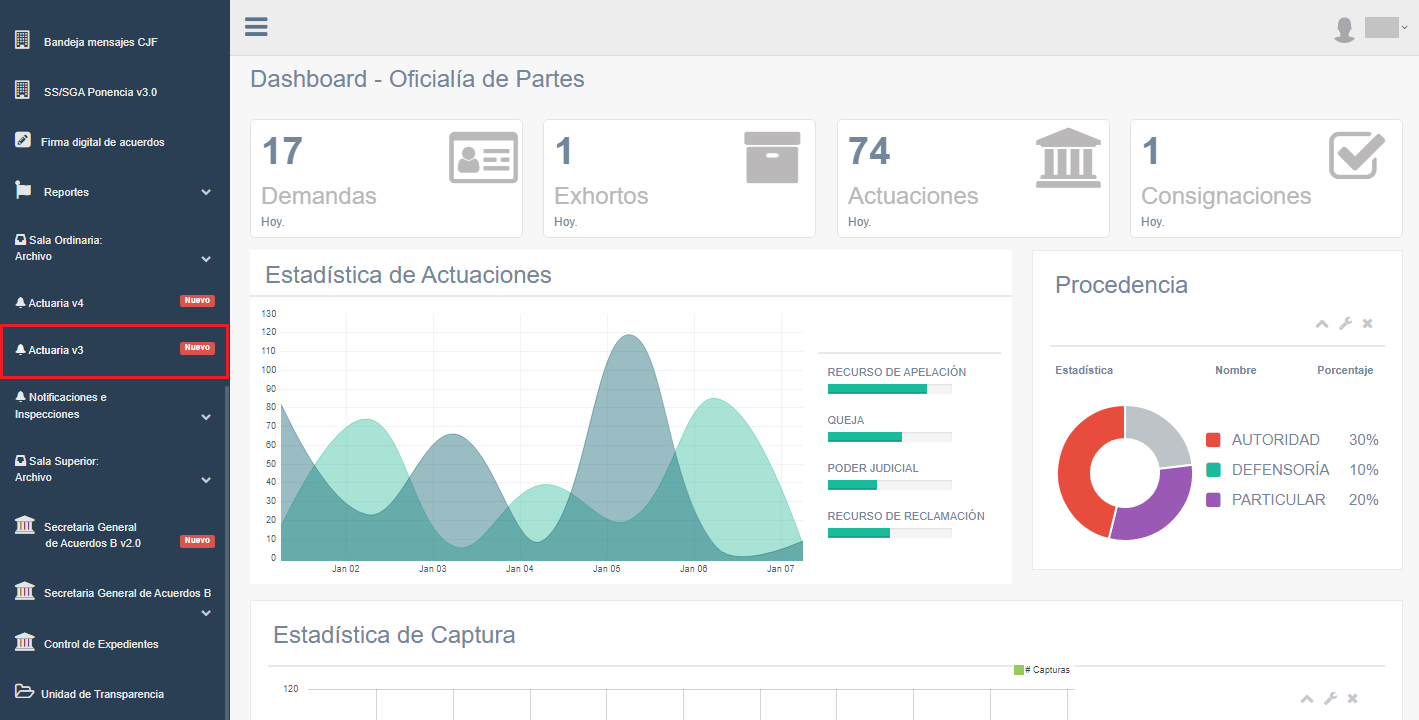
\includegraphics[width=0.88\columnwidth]{inicioAc.png}
\end{center}

\newpage

\chapter{\large{ Consulta de expediente y notificaciones.}}\label{chap:consulta}

En la sección  {\bf Consulta de expediente y notificaciones} podrá realizar las siguientes actividades:

\begin{itemize}
    \item Buscar expediente.
    \item Consulta de notificación.
    \item Subir notificación.
    \item Visualizar notificación.
    \item Editar notificación.
    \item Eliminar notificación.
    \item Buscar notificación.
\end{itemize}


\begin{center}
\begin{tabular}{| c | c | c | c | c}
\hline

\multicolumn{4}{ |c| }{\cellcolor[gray]{0.9} CONTROL DE VERSIONES} \\ \hline

\cellcolor[gray]{0.9} \bf Roles 
&\cellcolor[gray]{0.9} \bf Lectura 
& \cellcolor[gray]{0.9} \bf Escritura 
& \cellcolor[gray]{0.9} \bf Borrar 
\\ 
\hline
Admin & X & X & X \\ 
\hline
Actuario SO & X & X & X \\ 
\hline
Actuario SGA & X & X & X \\ 
\hline

\hline
\end{tabular}
\label{tab:versiones}
\end{center}
\newpage
{\color{myblue}\section{\normalfont\sffamily{Formas de buscar un expediente.}}}\label{sec:1.0}

Para poder buscar un expediente es necesario que siga la siguiente nomenclatura:
\begin{center}
    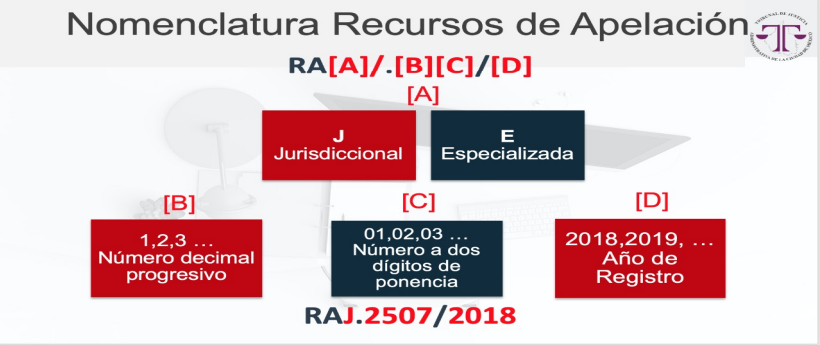
\includegraphics[width=0.77\columnwidth]{C1.png}
    
    \vspace{0.5cm}
    
    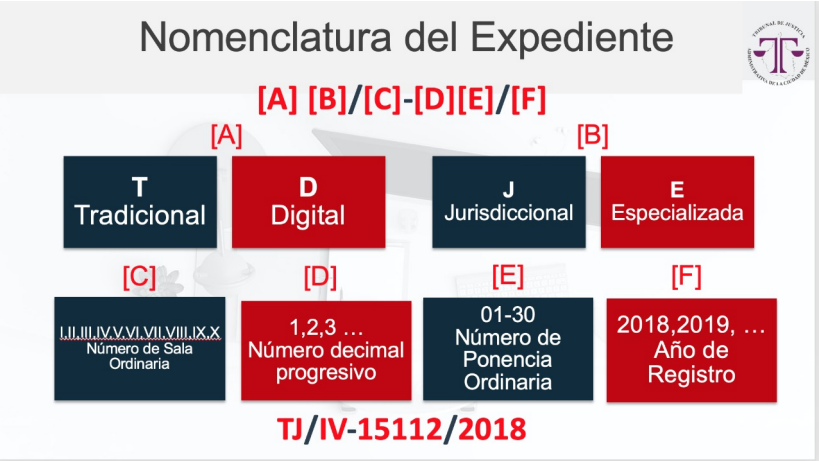
\includegraphics[width=0.77\columnwidth]{C2.png}
\end{center}

Ejemplos:
\begin{itemize}
    \item TJ/I-01/2018.
    \item -01/2018.
    \item RAJ.2507/2018.
    \item .2507/2018.
\end{itemize}

{\color{myblue}\section{\normalfont\sffamily{¿Cómo se consulta un expediente?}}}\label{sec:1.1}

Una vez que haya ingresado, a la opción {\bf «Consulta de expediente»}, verá una pantalla como la
siguiente, con los elementos mencionados a continuación:

\begin{center}
    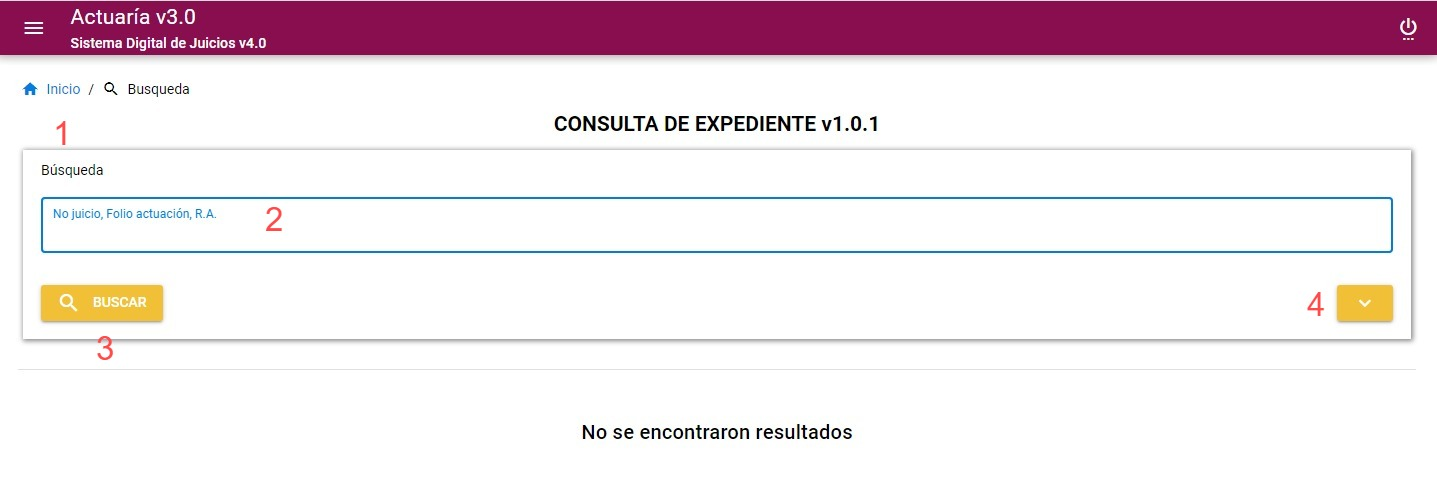
\includegraphics[width=0.88\columnwidth]{consulta.jpeg}
\end{center}
\begin{enumerate}
    \item Pulsando {\bf «Inicio»} podrá volver en cualquier momento a la pantalla de Inicio del aplicativo.
    \item No. juicio: en esta opción deberá ingresar el número de juicio para realizar la búsqueda.
    \item BUSCAR. Una vez que ingrese el número de juicio deberá dar clic en el botón {\bf «BUSCAR»} el
cual mostrará los resultados obtenidos.
    \item BUSQUEDA AVANZADA: Esta opción lo llevara a la pantalla de búsqueda avanzada.
\end{enumerate}


\begin{center}
    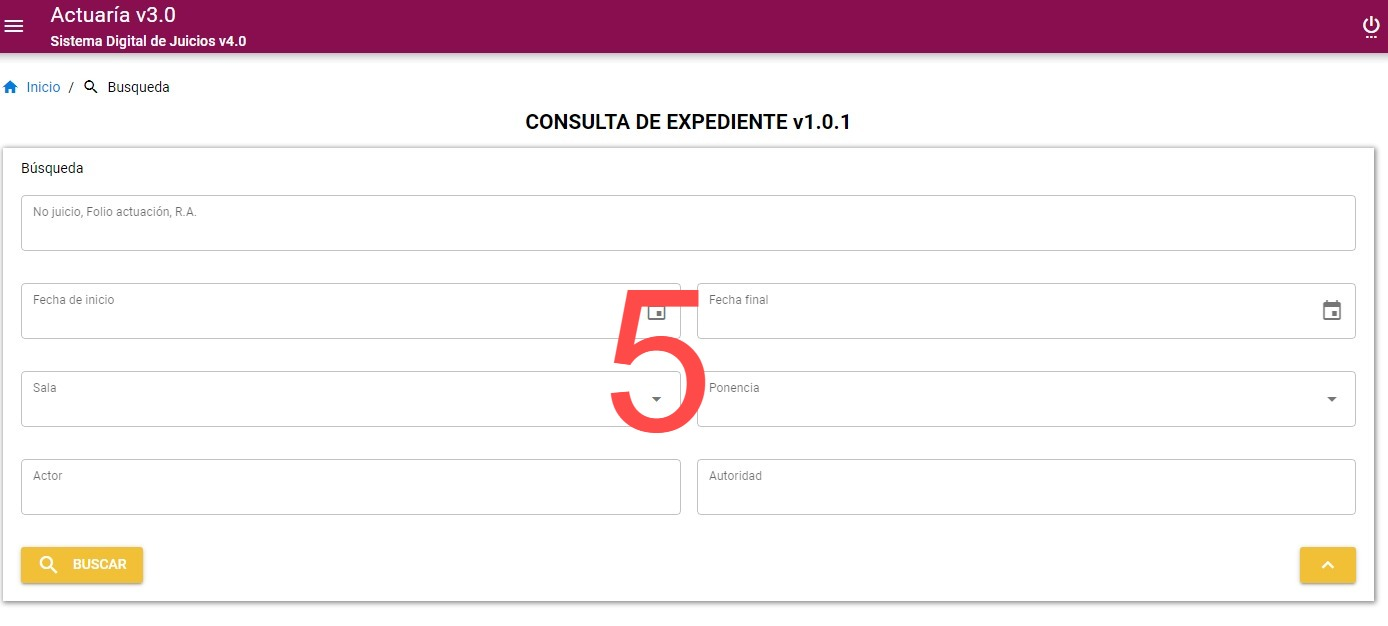
\includegraphics[width=0.88\columnwidth]{avanzada.jpeg}
\end{center}

5. Para realizar una búsqueda avanzada deberá contar con al menos uno de los siguientes
datos:
\begin{itemize}
    \item Sala.
    \item Ponencia.
    \item Actor.
    \item Autoridad.
    \item Fecha de inicio(ingreso de la actuación).
    \item Fecha final (Ingreso de la actuación).
\end{itemize}

\begin{center}
    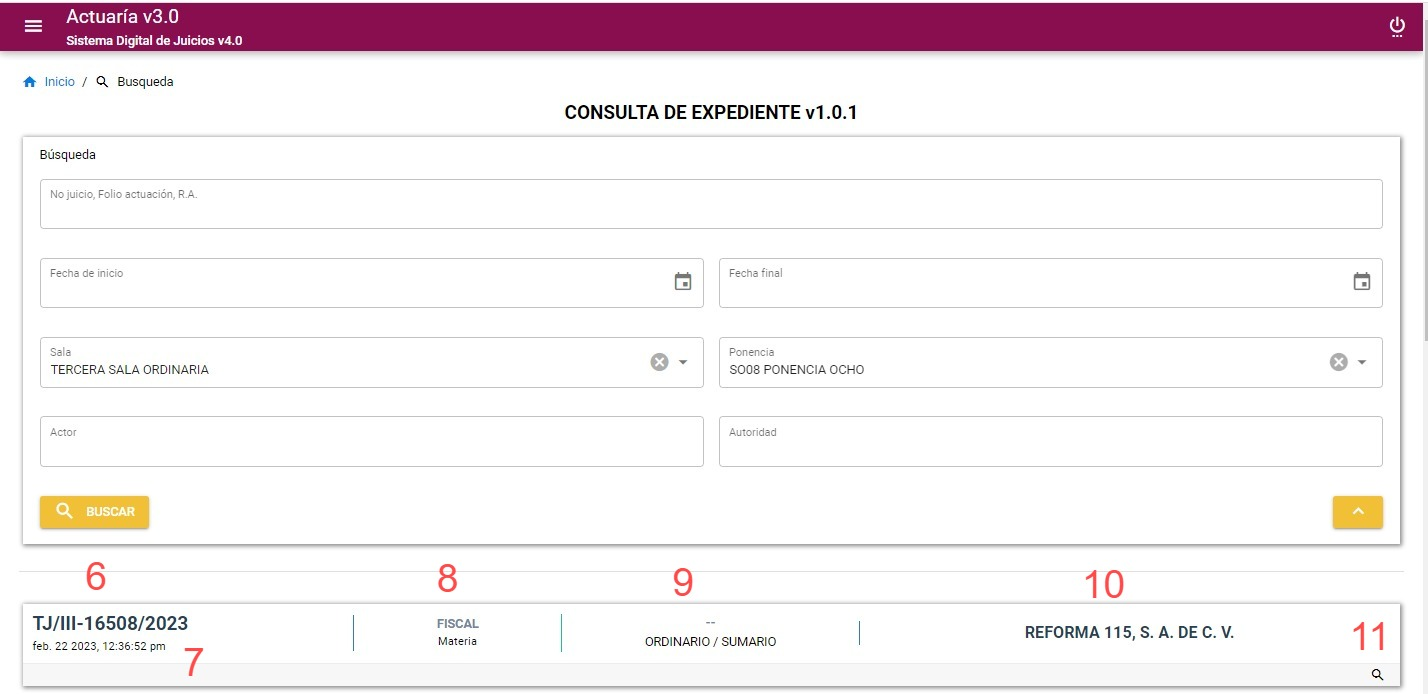
\includegraphics[width=0.88\columnwidth]{avanzada1.jpeg}
\end{center}

Una vez ingresado los datos para la búsqueda deberá dar clic el botón {\bf «BUSCAR»}, el cual mostrará
los resultados obtenidos, con la descripción de los elementos referidos a continuación:

\begin{enumerate}[ ]
    \item 6. Número de juicio.
    \item 7. Fecha ingreso.
    \item 8. Materia.
    \item 9. Ordinario/ Sumario.
    \item 10. Actor.
    \item 11. Consultar.
\end{enumerate}


Para poder ver toda la información del expediente es necesario dar clic en consultar, como se
muestra en la descripción anterior número 11, el cual presentará la siguiente pantalla.
Donde se podrá encontrar toda la información del expediente, a continuación, se describe los
elementos referidos a la consulta de expediente.

\begin{center}
    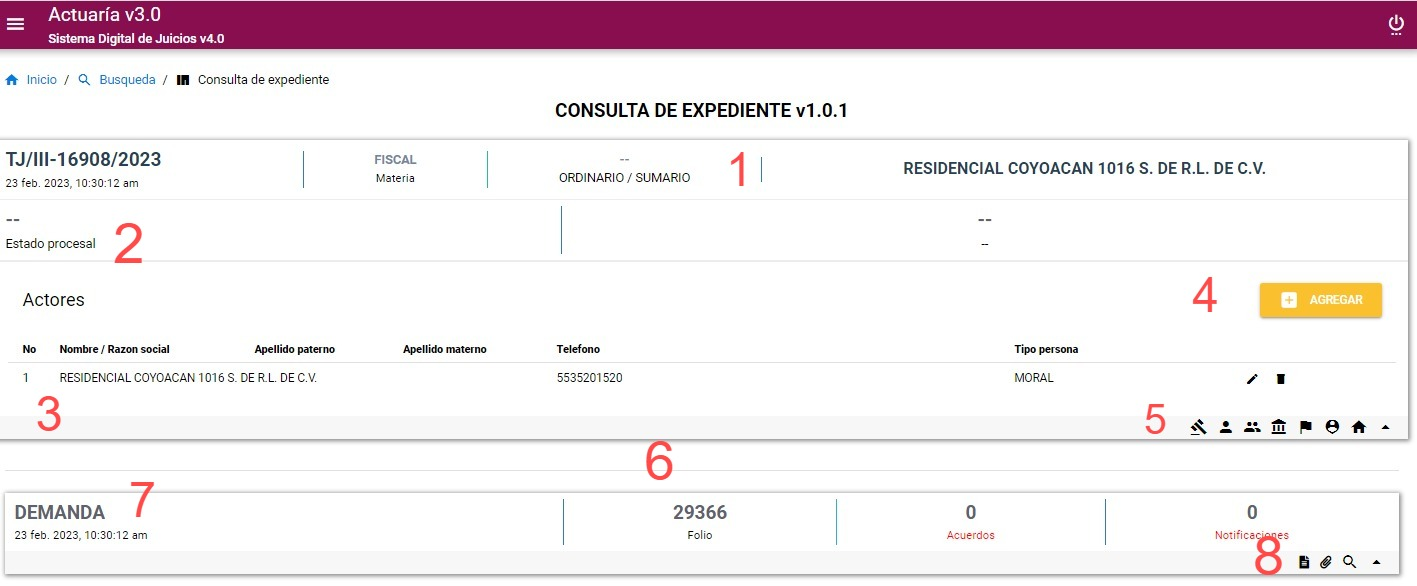
\includegraphics[width=0.88\columnwidth]{consulta_exp.jpeg}
\end{center}

1. Contenedor con Información de expediente:

\begin{itemize}
    \item Número de juicio.
    \item Fecha.
    \item Materia.
    \item Ordinario/Sumario.
    \item Actor.
\end{itemize}

2. Estado procesal.

3. Se podrá visualizar la información con solo dar clic un icono que están ubicados con el
número {\bf “5”}.

4. Agregar.

5. Iconos contenedores de expediente:
\begin{multicols}{2} %multicolumnas
\begin{itemize}
    \item Ponencia.
    \item Actores.
    \item Terceros perjudicados.
    \item Autoridades.
    \item Representantes.
    \item Autorizados.
    \item Domicilio.
\end{itemize}
\end{multicols}

6. Muestra la lista de actuaciones que tiene el expediente.

7. Contenedor de la actuación con la siguiente información:
\begin{itemize}
    \item Tipo de proceso.
    \item Fecha.
    \item Folio.
    \item Número de acuerdo.
    \item Número de notificaciones.
\end{itemize}

8. Iconos contenedor actuaciones:
\begin{itemize}
    \item Promociones.
    \item Anexos.
    \item Consultar.
\end{itemize}

\newpage

{\Huge{\color{myblue} \section{¿Cómo consultar una notificación?}\label{sec:1}}}

Es necesario dar clic en el icono {\bf «Consultar»} ubicado en el {\bf número “8”}, descrito anteriormente para
que pueda consultar una notificación.\\
Se mostrará los datos de la notificación, de clic en el icono {\bf {<<Visualizar>>}} ubicado en el {\bf{número ''1''}}.

\begin{center}
    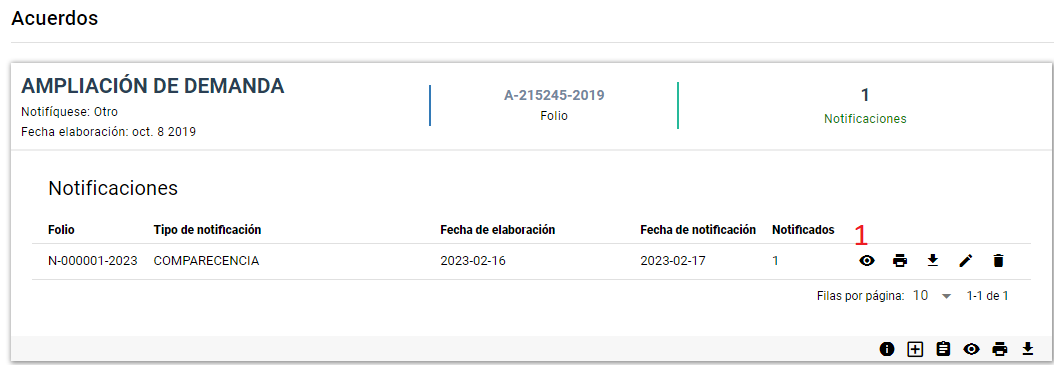
\includegraphics[width=0.88\columnwidth]{consultar_notificacion.png}
\end{center}

Se abrirá una ventana mostrando el documento.

\begin{center}
    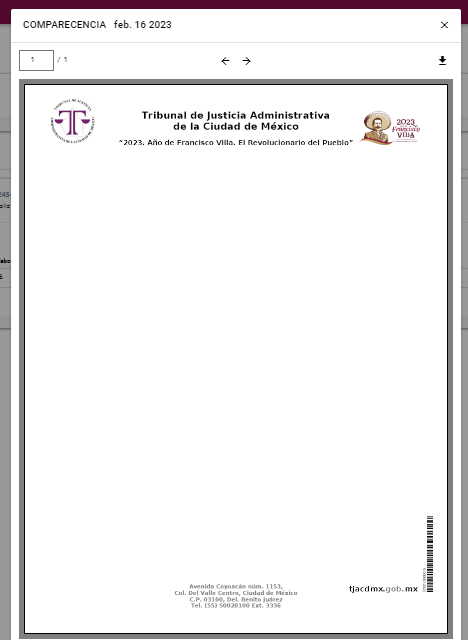
\includegraphics[width=0.40\columnwidth]{documento.png}
\end{center}

{\Huge{\color{myblue} \section{¿Cómo registrar una notificación?}\label{sec:2}}}

Es necesario dar clic en el icono {\bf«Consultar»} ubicado en el {\bf número 8}, descrito anteriormente para
que pueda subir una notificación. A continuación, se describe:

\begin{center}
    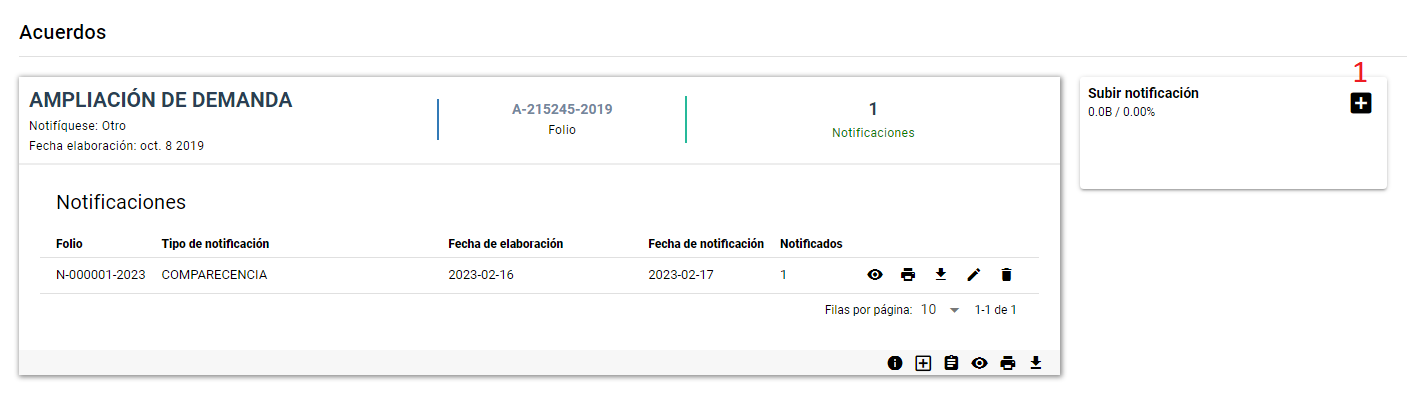
\includegraphics[width=0.88\columnwidth]{subir_notificacion.png}
\end{center}

De clic en el icono ubicado con el {\bf{ número 1}} podrá seleccionar el archivo donde este guardado el documento, 
una vez que seleccione el documento, deberá dar clic el botón abrir que mostrará la siguiente pantalla de
{\bf{''Registro de cédulas de notificación''}}

\begin{center}
    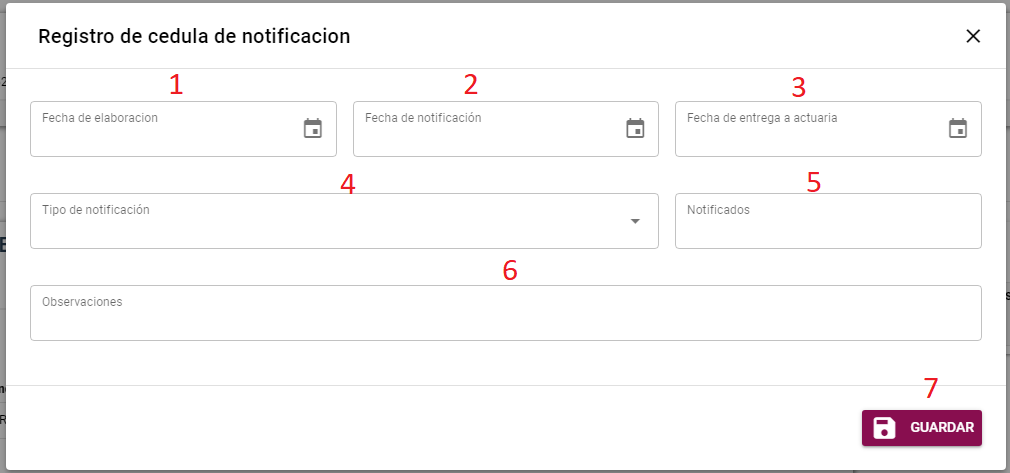
\includegraphics[width=0.55\columnwidth]{form_cedula.png}
\end{center}

Donde deberá ingresar la siguiente información:

\begin{multicols}{2} %multicolumnas
\begin{enumerate}[1.]
    \item Fecha de elaboración.
    \item Fecha de notificación.
    \item Fecha de entrega a actuaria
    \item Tipo de notificación.
    \item Notificados.
    \item Observaciones.
    \item Guardar
\end{enumerate}
\end{multicols}

Una vez capturada la información antes mencionada solo deberá dar clic el botón {\bf «Guardar»}
(ubicado en el lugar {\bf “número 7”}), mostrará la notificación registrada.
\newpage

{\color{myblue}\section{\normalfont\sffamily{¿Cómo editar una notificación?}}}\label{sec:3}

Es necesario dar clic el icono {\bf «Consultar»} ubicado en el {\bf “número 8”}, descrito anteriormente para
que pueda editar una notificación. A continuación, se describe.

\begin{center}
    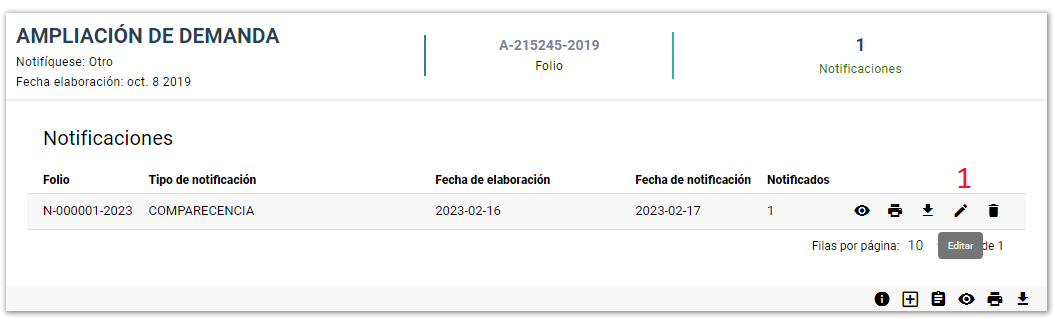
\includegraphics[width=0.88\columnwidth]{editar_notificacion.png}
\end{center}

Da clic en el icono <<Editar>> indicado con el {\bf{número ''1''}} abrirá la siguiente ventana mostrando la
información de notificación.

\begin{center}
    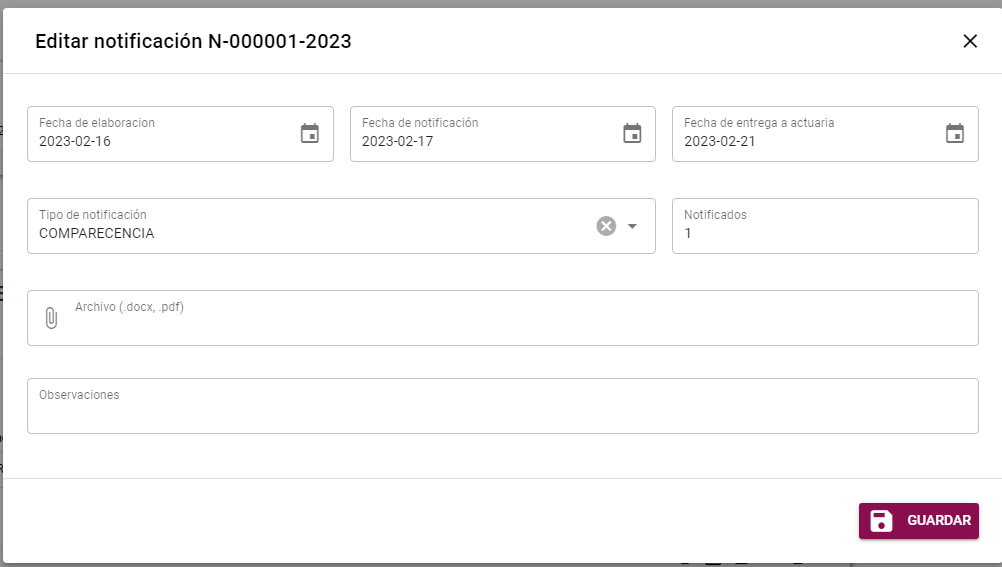
\includegraphics[width=0.65\columnwidth]{editar_not.png}
\end{center}

Podrá modificar toda la información e incluso volver a subir el archivo de notificación y podrá
guardar los cambios pulsando el botón {\bf «Guardar»}.
\vspace{3cm}
{\Huge{\color{myblue} \section{¿Cómo borrar una notificación?}\label{sec:4}}}

Es necesario dar clic el icono «Consultar» ubicado en el “número 8”, descrito anterior-
mente para que pueda borrar una notificación. A continuación, se describe:

\begin{center}
    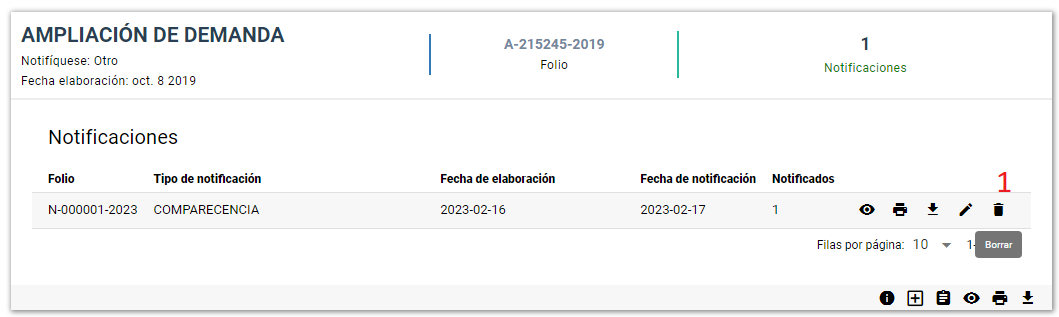
\includegraphics[width=0.65\columnwidth]{borrar_not.png}
\end{center}

Da clic en el icono «Borrar» indicado con el {\bf{número ”1”}} que mostrará una ventana de advertencia.

\begin{center}
    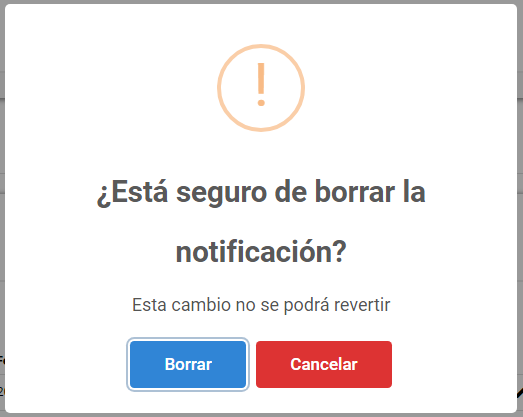
\includegraphics[width=0.33\columnwidth]{advertencia.png}
\end{center}

Sí está seguro de eliminar confirme en el botón {{\bf<<Borrar>>}} de lo contrario solo dar clic en {{\bf<<Cancelar>>.}}


{\Huge{\color{myblue} \section{¿Cómo descargar una notificación?}\label{sec:5}}}

Es necesario dar clic el icono {\bf{«Consultar»}} ubicado en el {\bf{“número 8”}}, 
descrito anteriormente para que pueda borrar una notificación. A continuación, se describe:

\begin{center}
    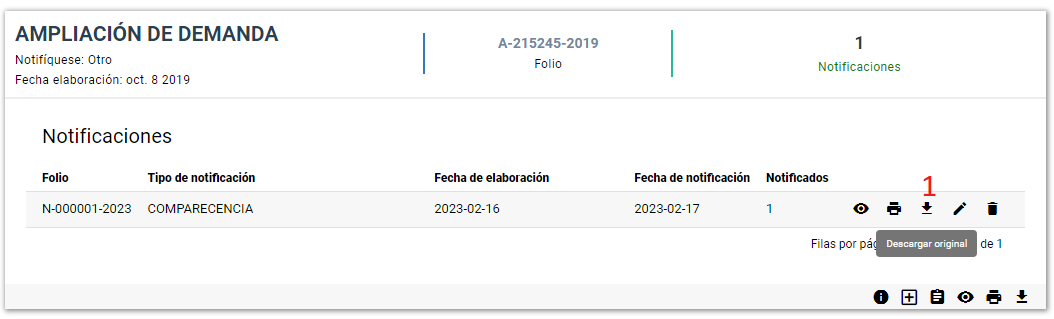
\includegraphics[width=0.88\columnwidth]{descargar_not.png}
\end{center}

Da clic en el icono «Descargar» indicado con el número ”1”, y comenzará automáticamente la descarga.

\newpage
\begin{table}[t]
\begin{center}
\begin{tabular}{| c | c | c | c | }
\hline

\multicolumn{4}{ |c| }{\cellcolor[gray]{0.9}CONTROL DE VERSIONES}
\\ \hline
Versión
& Elaborado por:
& Fecha de última modificación
& Motivo
\\ \hline

1.0.1
& Esthefania Vidal
& 03/01/2023
&Creación
\\ \hline

1.0.1
& Esthefania Vidal
& 28/02/2023
&Actualización
\\ \hline
\end{tabular}
\caption{Control de versiones}
\end{center}
\end{table}


\newpage


\end{quote}

\end{document}



